\documentclass[a4paper]{article}
\usepackage[T1]{fontenc}
\usepackage[margin=1in]{geometry}
\usepackage{listings}
\usepackage{xcolor}
\usepackage{courier}
\usepackage{graphicx}
\usepackage{hyperref}
\usepackage{sidecap}
\usepackage{wrapfig}
\usepackage{subfig}
\usepackage{float}
\renewcommand{\figurename}{Rysunek}

\lstdefinestyle{sharpc}{language=[Sharp]C, frame=lr, rulecolor=\color{blue!80!black}}

\title{Cechy sygnału audio w dziedzinie częstotliwości\\
\large Projekt nr 3 - Analiza i Przetwarzanie Dźwięku\\ 
\small \url{https://github.com/szymon159/sound-analysis}}
\date{}
\author{Szymon Stasiak}

\begin{document}
  \maketitle

\section{Opis aplikacji}
Projekt stworzony został w .NET Framework, z warstwą prezentacji powstałą w Windows Forms i interfejsem w języku angielskim. Analiza wspiera pliki \textit{*.wav} oraz \textit{*.mp3}.\\
Jest to rozwinięcie projektów \textit{Cechy sygnału audio w dziedzinie czasu} oraz \textit{Analiza częstotliwościowa dźwięku}, dodające do poprzednich wersji nową opcje widoku - parametry w dziedzinie częstotliwości \textbf{Frequency Parameters} oraz pola \textbf{Band Start} i \textbf{Band End} wykorzystywane w liczeniu \textit{Band Energy}\\
W celu uproszczenia obliczeń używane są również zewnętrzne paczki (żadnych zmian w stosunku do poprzedniego projektu):
\begin{itemize}
\item \textit{NAudio} - w celu wczytywania, parsowania i podstawowych operacji na plikach
\item \textit{MathNet.Numerics} - dostarcza narzędzia do obliczania transformaty Fouriera oraz stosowania funkcji okienkowych
\item \textit{Oxyplot} - usprawnienie wykresów
\end{itemize}
Jako nagrania testowe posłużyły nagrania stworzone na potrzeby przedmiotu (\textit{Rysunki 1, 2 i 3}), a ponadto: fragment przemówienia Baracka Obamy (jako przykład mowy, pobrany ze strony \url{http://soundbible.com/}) - \textit{Rysunki 4} oraz \textit{6} oraz fragment utworu \textit{Adventure} stworzony przez Bensound (jako przykład muzyki instrumentalnej udostępniony za darmo na stronie \url{https://www.bensound.com/royalty-free-music/}) - \textit{Rysunki 5} oraz \textit{7}.
\subsection{Głowne okno programu}
Główne okno programu uległo nieznacznej zmianie w stosunku do poprzedniego projektu. Dodana została zakładka \textit{Frequency Parameters} z nowymi parametrami, pozostałe zakładki wciąż przedstawiają parametry obliczone w poprzednich projektach.
\begin{figure}[H]
  \centering
  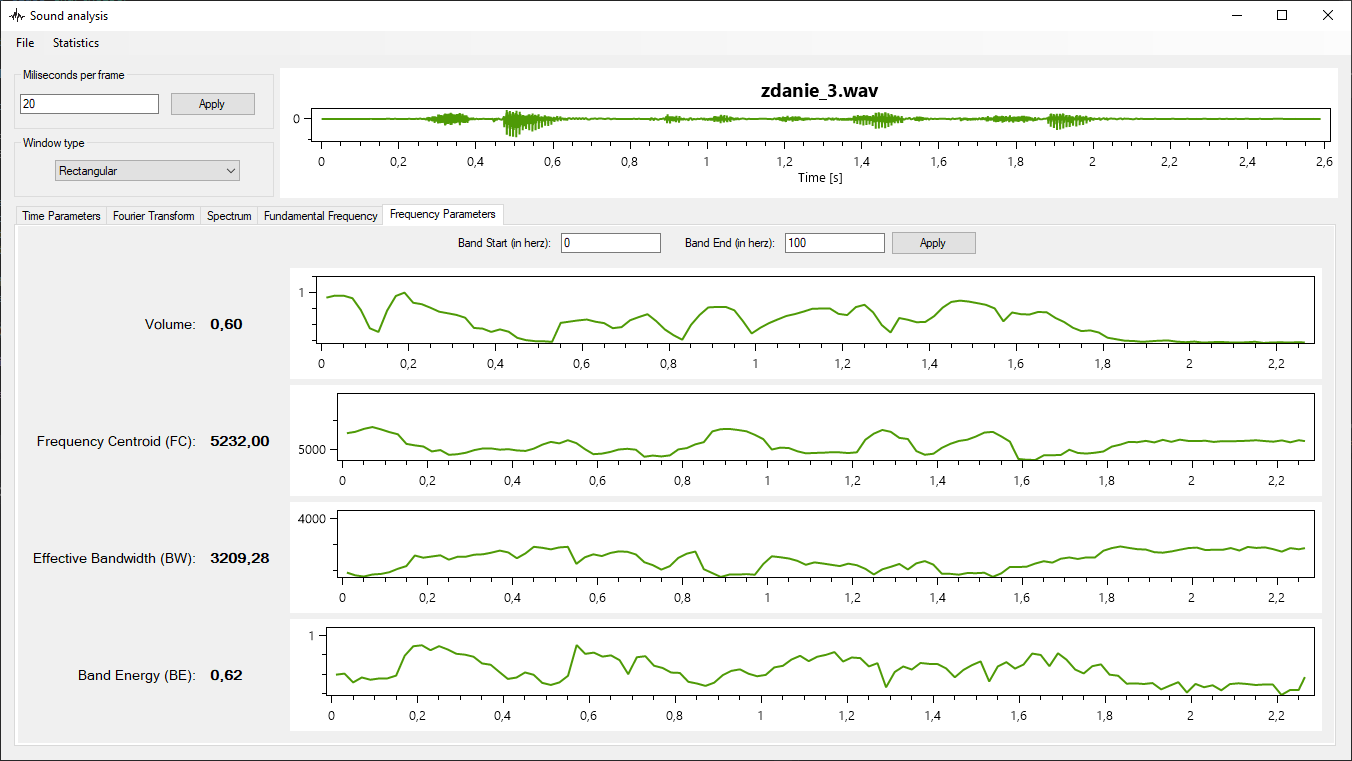
\includegraphics[width=0.75\linewidth]{images/01interface.png}
  \caption{Interfejs programu}
\end{figure}
\noindent Parametry obok wykresów oznaczają średnią z wartości dla wszystkich ramek nagrania.

\section{Opis metod}
\subsection{Cechy na poziomie ramki (Frame-level)}
Ilość ramek wyliczana jest na podstawie podanej wartości milisekund na ramkę (\textit{Miliseconds per frame}, lewy górny róg) oraz pobranej przy wczytywaniu pliku częstotliwości próbkowania.\\
Na wszystkich wykresach wartość dla ramki zaznaczona jest w jej środku. W przypadku nierównego podziału, ostatnia ramka może być dużo krótsza niż pozostałe (jednak punkt wciąż zaznaczony jest w jej środku).\\
W odróżnieniu od obliczeń w dziedzinie czasu, punktem wyjścia do analizy częstotliwościowej jest wynik transformaty Fouriera. Z tego powodu możliwa jest również zmiana okna używanego przy stosowaniu transformaty (co z kolei wpływa na wyniki).\\
We wszystkich wzorach z tego rozdziału zachowane zostało następujące znaczenie symbol: \textit{$n$} - kolejny indeks ramki, \textit{$N$} - długość ramki w próbkach, \textit{$S_n(k)$} - wartość dla $k$-tej (obliczonej z pomocą transformaty Fouriera) częstotliwości w $n$-tej ramce.\\
Ponadto poniższe omówienie wszystkich cech zawiera odwołania do przykładowych nagrań (zarówno nieznormalizowanego jak i znormalizowanego). W celu uproszczenia odbioru, \textit{Rysunek 2} oraz \textit{Rysunek 3} prezentują jedno przykładowe nagranie w obu tych wariantach.
\begin{figure}[H]
  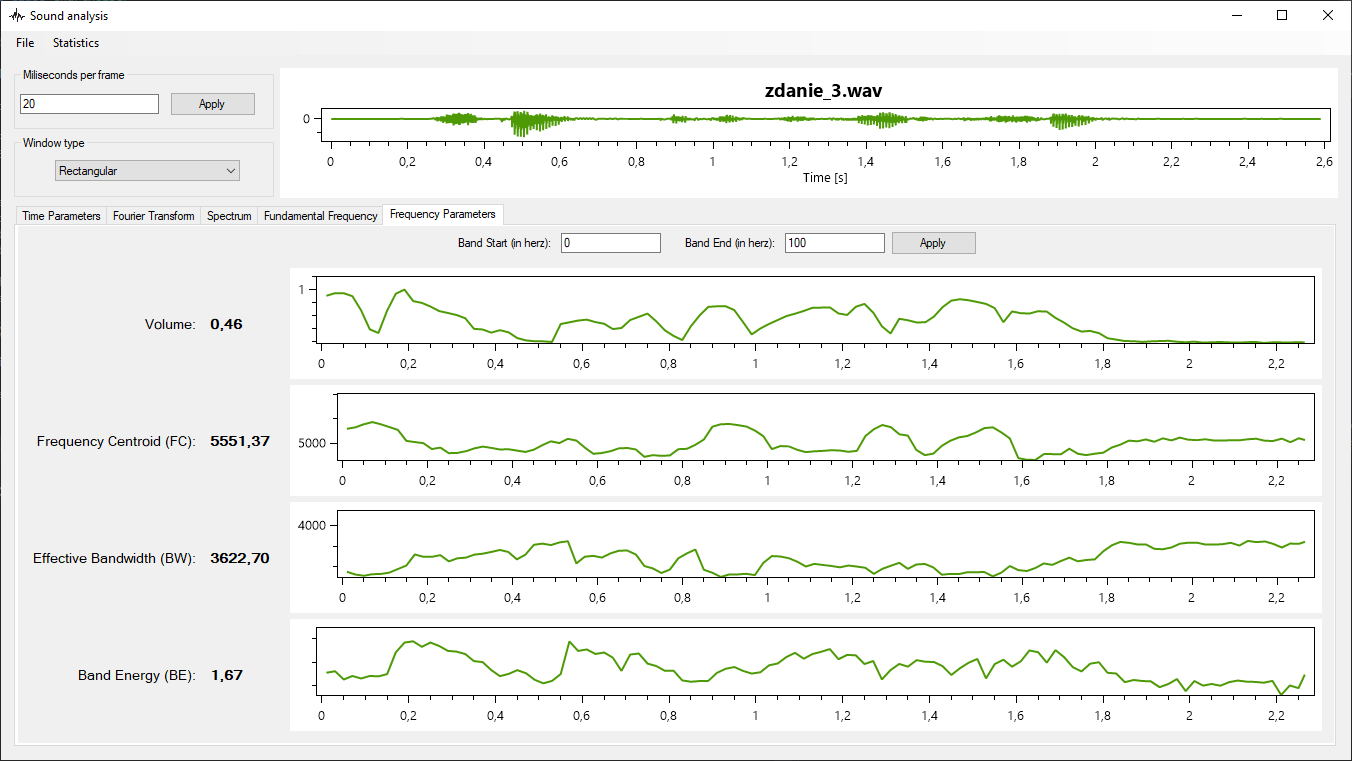
\includegraphics[width=\linewidth]{images/02notnormalized.png}
  \caption{Nienznormalizowane nagranie}
\end{figure}
\begin{figure}[H]
  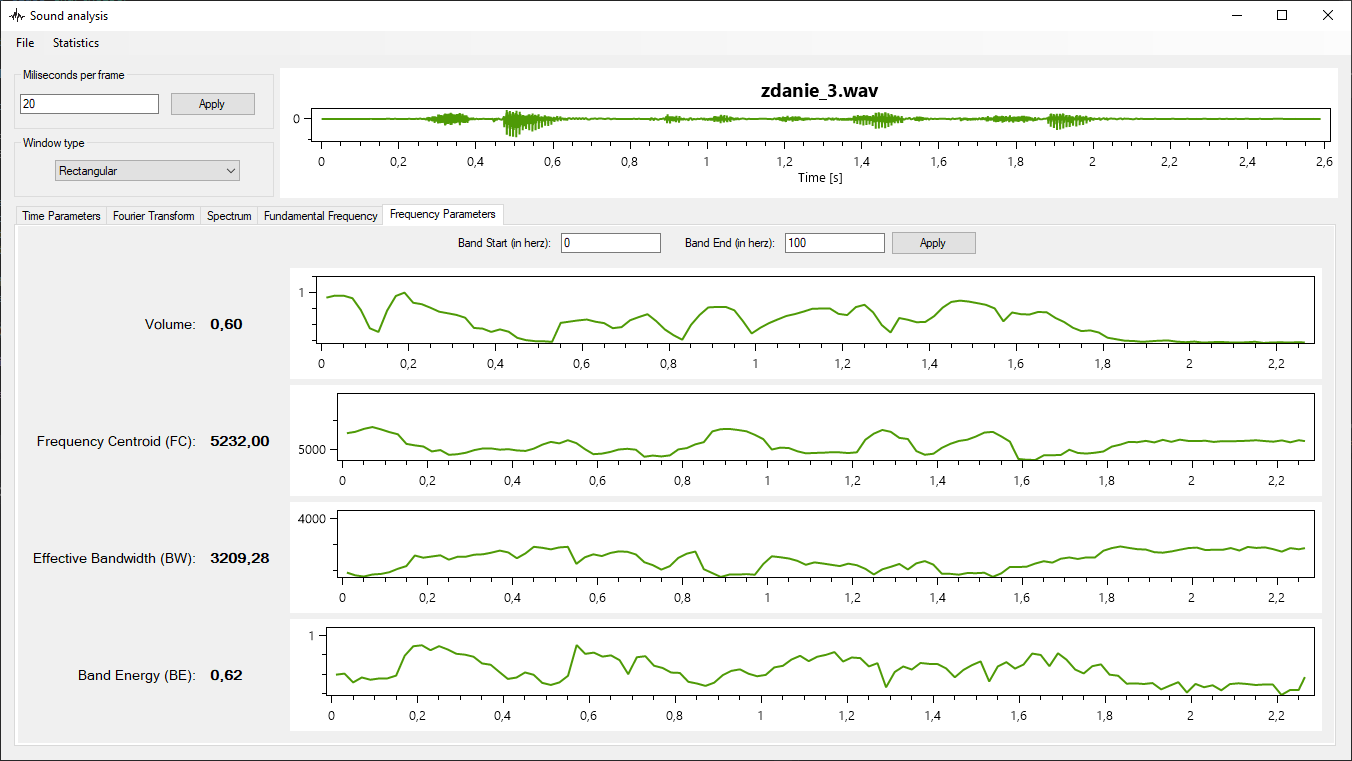
\includegraphics[width=\linewidth]{images/03normalized.png}
  \caption{Znormalizowane nagranie}
\end{figure}

\subsubsection{Głośność (Volume)}
Wartość głośności dla każdej klatki wyliczana jest zgodnie ze wzorem dostępnym w materiale źródłowym, czyli:
\begin{equation}
Volume(n) = \frac{1}{N} \sum_{k=0}^{N-1}S_n^2(k)
\end{equation}
Podobnie jak w przypadku analizy w dziedzinie czasu, widoczny jest wpływ normalizacji na głośność nagrania. W analizowanym przypadku, nagranie znormalizowane jest głośniejsze od nieznormalizowanego. Widać to jednak wyłącznie poprzez wartość średnią, gdyż sam kształt wykresu dla obu wersji jest niemal identyczny. Nieznaczne różnice wynikają częściowo z błędów zaokrągleń spowodowanych wielokrotną transformacją wczytanych wartości (w szczególności zastosowaną transformatą Fouriera).

\subsubsection{Centrum częstotliwości (Frequency Centroid)}
Analiza komputerowa w dziedzinie częstotliwości jest analizą dyskretną. Z tego też powodu we wzorze służącym do obliczenia analizowanego parametru całka została zastąpiona sumą (a więc miara analityczna zastąpiona miarą numeryczną). Powstały wzór ma zatem postać:
\begin{equation}
FC(n) = \frac{\sum_{k=0}^{N-1}k*S_n(k)}{\sum_{k=0}^{N-1}S_n(k)}
\end{equation}
Wartość tego parametru jest używana do odróżnienia mowy od ciszy oraz muzyki od mowy. Wyniki przedstawione są w następnej sekcji \textit{3 Wyniki działania}.

\subsubsection{Efektywne pasmo (Effective Bandwidth)}
Podobnie jak w przypadku poprzedniego parametru, także w przypadku pasma należy przekształcić wzory do postaci dyskretnej. Dodatkowo warto odnotować iż wartość tego parametru w każdej ramce jest zależna od wyliczonego uprzednio centrum (oznaczonego przez $FC(n)$). Po podstawieniu odpowiednich symboli, używany wzór ma postać:
\begin{equation}
BW(n) = \sqrt{\frac{\sum_{k=0}^{N-1}[(k-FC(n))*S_n(k)]^2}{\sum_{k=0}^{N-1}S_n^2(k)}}
\end{equation}
Zastosowanie wyliczonej wartości pasma jest zbliżone do centroidu - tak jak on pozwala odróżniać mowę od muzyki oraz ciszę od mowy.

\subsubsection{Energia (Band Energy)}
Ostatnim z analizowanych parametrów jest energia określonego pasma częstotliwości. W tym przypadku, do analizy dochodzą dwa dodatkowe parametry $f_0$ oraz $f_1$ - odpowiednio oznaczające początek i koniec zakresu pasma. Są one konfigurowalne jako liczby całkowite z poziomu interfejsu aplikacji. Po dodaniu tych wartości i przejściu do postaci dyskretnej otrzymany wzór ma postać:
\begin{equation}
BE_{[f_0, f_1]}(n) = \frac{\sum_{k=k_0}^{k_1}S_n^2(k)}{\sum_{l=0}^{N-1}w(l)}
\end{equation}
We wzorze pojawiają się jeszcze trzy nieopisane wcześniej symbole: $k_0$, $k_1$ oraz $w(l)$. Pierwsze dwa oznaczają indeksy próbek którym odpowiadają częstotliwości pasma: odpowiednio $f_0$ oraz $f_1$. Z kolei $w(l)$ oznacza wartość $l$-tej próbki wczytanego nagrania (przed przejściem do dziedziny częstotliwości).\\
Wartość energii również może być z powodzeniem używana w detekcji mowa-muzyka.

\section{Wyniki działania}
Szczególnie istotnymi aspektami projektu, na których warto się skupić jest, podobnie jak w przypadku parametrów w dziedzinie czasu, odróżnianie muzyki od mowy.\\
Testowymi nagraniami były już wspomniane nagrania korpusu tekstowego, jednak z powodu braku muzyki analizie zostały poddane również inne pliki źródłowe.
\subsection{Normalizacja nagrań}
Na samym początku warto poświęcić chwilę analizie różnic między nagraniami nieznormalizowanymi a znormalizowanymi. Jako przykład może tutaj posłużyć porównanie \textit{Rysunku 2} oraz \textit{Rysunku 3} wspomnianych w sekcji \textit{2 Opis metod}. Delikatne różnice między parametrami są widoczne szczególnie w zakresie wartości. Często wynika to z kumulacji błędów zaokrągleń - wartości znacznie mniejsze od 0 zostają poddane transformacie Fouriera a następnie wielokrotnie wykonywane są na nich obliczenia takie jak pierwiastek czy mnożenie.\\
Warto jednak zauważyć, że dla nagrania nieznormalizowanego wyłącznie głośność osiąga wartości mniejsze niż dla znormalizowanego. W przypadku pozostałych parametrów sytuacja jest odwrotna - wartości większe osiągane są przez nagranie znormalizowane.

\subsection{Mowa a muzyka}
Niestety nagrania stworzone na potrzeby przedmiotu nie dają możliwości porównania mowy i muzyki. Z tego powodu, analizie poddane zostaną: zapowiedziany we wstępie fragment przemówienia Baracka Obamy (\textit{Rysunek 4} i \textit{6}) oraz utwór instrumentalny (\textit{Rysunek 5} i \textit{7}).\\
Niestety, wyniki przedstawionej na następnej stronie analizy są rozczarowujące. Można było oczekiwać iż wartości \textit{frequency centroid} oraz \textit{effective bandwidth} będą znacznie mniejsze dla mowy niż dla muzyki, tym czasem wartości te są niemal równe.
\begin{figure}[H]
  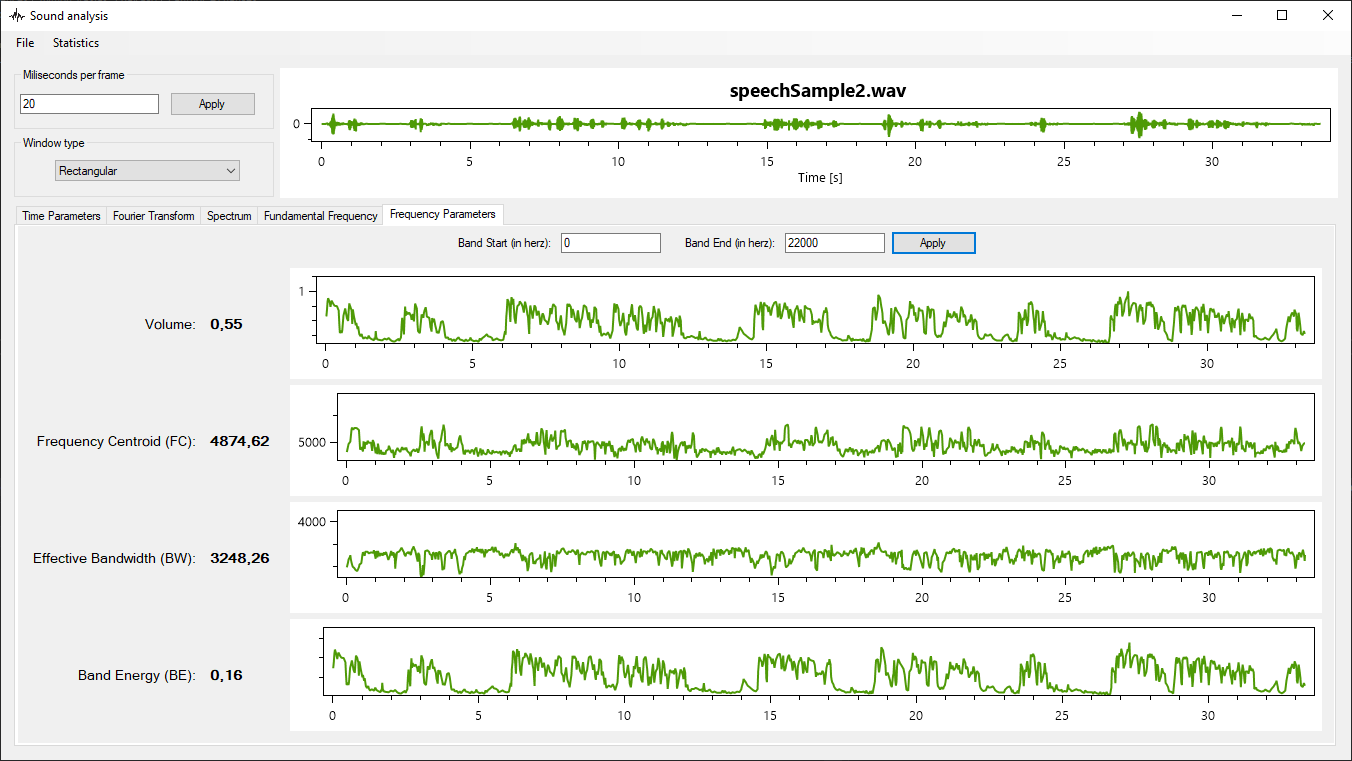
\includegraphics[width=\linewidth]{images/04speech.png}
  \caption{Fragment przemówienia Baracka Obamy}
\end{figure}
\begin{figure}[H]
  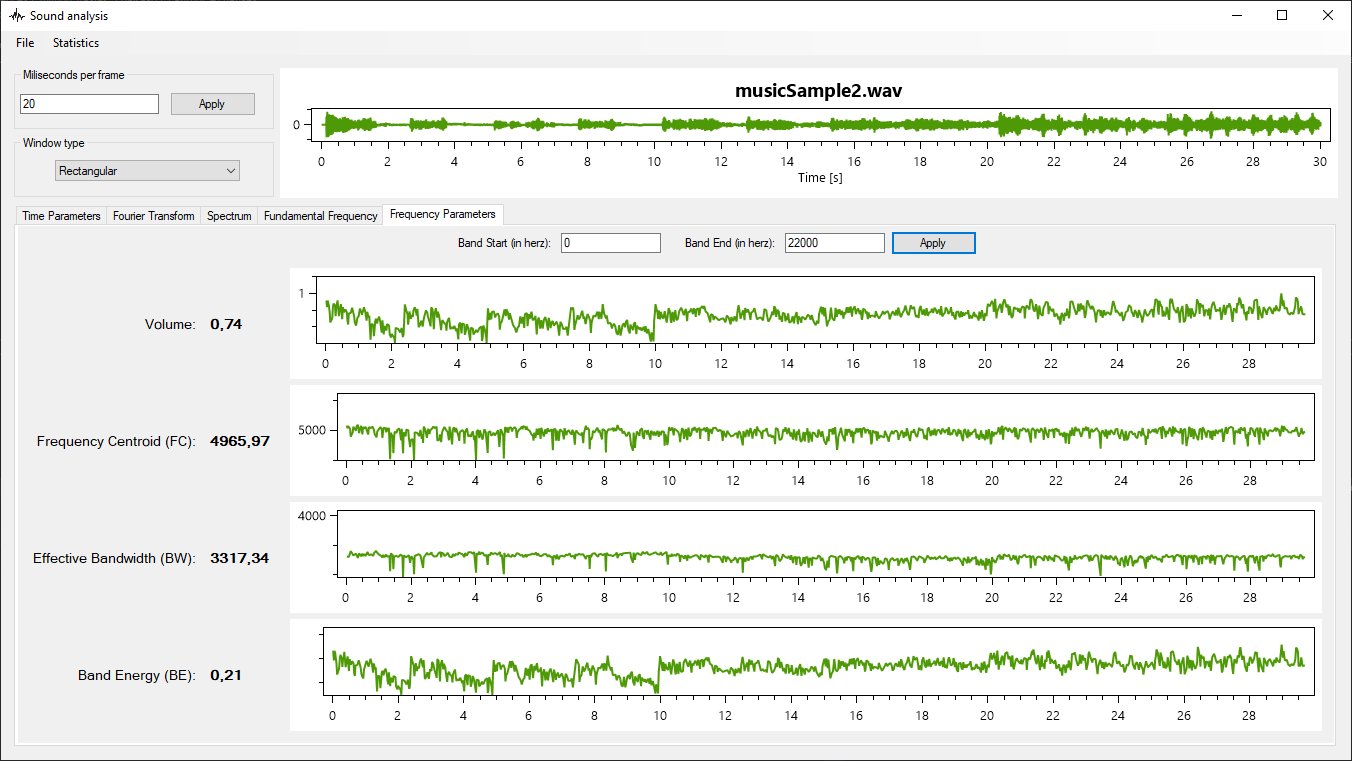
\includegraphics[width=\linewidth]{images/05music.png}
  \caption{Fragment muzyki z utworu \textit{Adventure} stworzonego przez Bensound}
\end{figure}
\noindent Sytuacja wygląda nieco lepiej dla analizy parametru \textit{band energy}. W tym przypadku, zgodnie z oczekiwaniami, wartość dla muzyki jest większa niż dla mowy. Dodatkowo energia w pasmie $0-500\:Hz$, a więc charakterystycznym dla mowy, jest wyższa niż dla całego pasma.
\begin{figure}[H]
  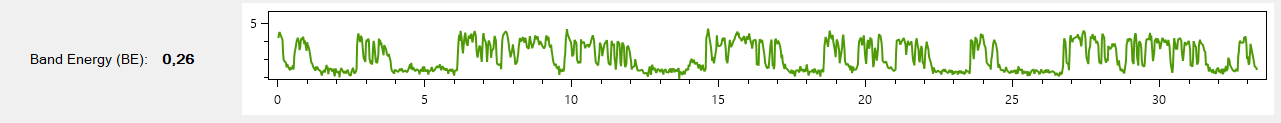
\includegraphics[width=\linewidth]{images/06speechEnergy.png}
  \caption{Energia w pasmie $0-500\:Hz$ dla nagrania mowy}
\end{figure}
\begin{figure}[H]
  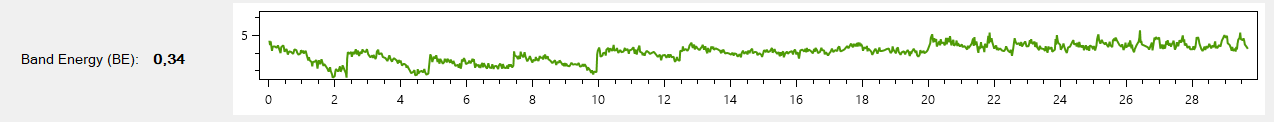
\includegraphics[width=\linewidth]{images/07musicEnergy.png}
  \caption{Energia w pasmie $0-500\:Hz$ dla nagrania muzyki}
\end{figure}
\noindent Kolejny aspekt przy którym wyznaczone parametry mogą okazać się pomocne, to odróżnianie fragmentów udźwiękowionych od ciszy. W tym przypadku efekty również są względnie zadowalające - dla przykładowej mowy fragmenty ciszy pokrywają się z niskimi wartościami parametrów \textit{frequency centroid} czy \textit{band energy}.

\section{Wnioski}
Parametry określane przez program niestety nie są wystarczająco dokładne aby jednoznacznie odróżnić na ich podstawie nagranie mowy i muzyki. Co prawda subtelne różnice między takimi nagraniami są widoczne, jednak wartości pozostawiają w tej kwestii wiele do życzenia. Z przedstawionej analizy wynika, iż najlepszym parametrem do tego typu klasyfikacji jest \textit{band energy}, jednak różnice są zdecydowanie za małe aby metoda ta była uznana za bezbłędną czy nawet godną zaufania.\\
Pozytywnie można jednak ocenić odróżnianie fragmentów udźwiękowionych od ciszy, co jest jednak niewielkim pocieszeniem gdyż istnieje wiele prostszych, szybszych, a przede wszystkim skuteczniejszych metod.

\lstset{basicstyle=\ttfamily}
\lstset{style=sharpc}
\begin{lstlisting}
\end{lstlisting}

\end{document}